\textbf{COLUNI 2021 -- Questão 23}\par\medskip A aceleração de um corpo tem a mesma direção e sentido da força resultante que atua sobre ele. Além disso, a aceleração informa quão rapidamente varia a velocidade do corpo. Pedro realizou um experimento em uma piscina, utilizando uma bola de borracha cheia de ar, como ilustra a figura abaixo. Inicialmente, ele segurou a bola, mantendo-a parada, na posição mostrada na figura. Em seguida, ele soltou-a e observou o seu movimento de subida em direção à superfície da água.

\par

% COLUNI-AUTO-FIGURES-BEGIN
\begin{figure}[htbp]
\centering
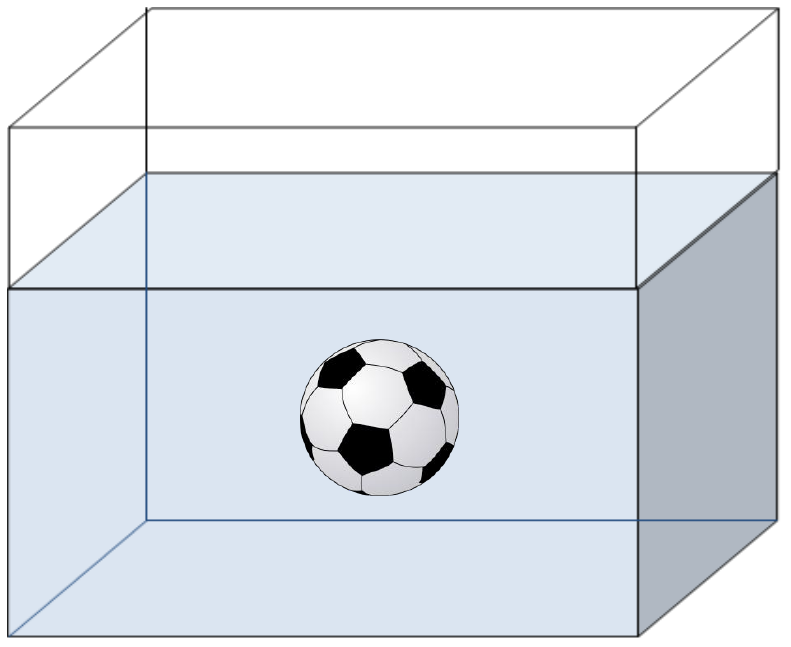
\includegraphics[width=0.95\linewidth]{static/simulados/coluni/figuras/2021/questao-23/figura-1.png}
\end{figure}
% COLUNI-AUTO-FIGURES-END

É CORRETO afirmar que, durante a subida, antes da sua parte superior atingir a superfície, a velocidade da bola:

\begin{enumerate}
\item primeiro aumentou e depois tornou-se constante.
\item primeiro aumentou e depois passou a diminuir.
\item aumentou o tempo todo.
\item manteve-se constante.\end{enumerate}
